% -- Introduction ---------------------------------------

\section{Introduction}

For the lab a computational intensive kernel has to be extracted from a \mcode{x264} software application, free software library for encoding video stream into H.236/MPEG-4 AVC format. The application is executed on a FPGA running a MicroBlaze host processor. By running the particular kernel on $\rho$-VEX co-processor, the execution time can be decreased by making use of hardware acceleration. 

\subsection{Getting Used to the Environment}
The first lab is meant to get used to the project environment. A few input files are given to show the compile and run commands of the x264 application, by inserting a \mcode{.y4m} stream and creating a short \mcode{.mkv} movie. By adding the \mcode{gprof} flag to the compile command, a list is created of all functions ordered by their share of the total execution time (in percentage). 

\subsection{Detecting the Computationally Most Intensive Kernel}

Profiling the x264 execution for the \mcode{.y4m} files that are provided by the lab leads to the ranking show in table \ref{tab:chart}.

\begin{table}[htb]%
\centering
	\begin{tabular}{lcll}
		\centering
		\bf{Input fie} & \bf{Execution time (in sec)} & \bf{Share (in $\%$)} & \bf{Kernel name} \\ \cline{1-4}
		\multirow{3}{*}{eledream\_32x18\_1.y4m}	&				& 100.00	& x264\_analyse\_init\_costs\\ 
																						&	0.02	& 0.00 		& x264\_free\\ 
																						&				& 0.00		& x264\_cabac\_encode\_desicion\_c\\ \cline{1-4}
		\multirow{3}{*}{eledream\_64x32\_3.y4m} & 			& 66.67		& x264\_analyse\_init\_costs\\
																						&	0.03	& 33.33 	& x264\_pixel\_satd\_4x4\\ 
																						&				& 0.00		& x264\_pixel\_satd\_8x4\\ \cline{1-4}
		\multirow{3}{*}{eledream\_640x320\_8.y4m}	& 			& 14.29	& x264\_pixel\_satd\_8x4\\ 
																							&	1.61	& 11.80 	& x264\_get\_ref\\ 
																							&				& 4.97		& x264\_pixel\_satd\_x4\_16x16\\ \cline{1-4}
		\multirow{3}{*}{eledream\_640x320\_32.y4m}& 			& 20.61	& get\_ref\\ 
																							& 8.54	& 13.23 	& x264\_pixel\_satd\_8x4\\ 
																							&				& 4.57		& x264\_pixel\_satd\_x4\_8x8\\ \cline{1-4}
		\multirow{3}{*}{eledream\_640x320\_128.y4m}&			& 17.48	& get\_ref\\
																							&	 29.86& 14.17 	& x264\_pixel\_satd\_8x4\\
																							&				& 6.56		& x264\_pixel\_satd\_x4\_16x16\\ \cline{1-4}
	\end{tabular}	

\caption{Chart with computationally most intensive kernels for each input stream.}
\label{tab:chart}
\end{table}

Given these statistics, we decide to extract the \mcode{x264\_pixel\_satd\_8x4 kernel}, since its share in execution time increases as the files become larger. This kernel evaluates the Sum of Transformed Differences between a 8x4 pixel block from the input stream and reference blocks using 4x4 transform (Hadamard???). DE EXECUTIETIJD IS VARIABEL, ELKE KEER DAT IK UITVOER MET GPROF OF TIME GEEFT IE ANDERE EXECUTIETIJDEN. DIT GETAL IS DUS NIET NAUWKEURIG.

\subsection{Executing an Application on the Development Board and $\rho$-VEX}

When executing \mcode{./configure}, a file is created for configuration of the application. However, the resulting \mcode{config.mak} file is made for applications running on the guest (Ubuntu). In order to configure for MicroBlaze, the \mcode{config.mak} file has to altered. All references to \mcode{m32} have to be removed and the \mcode{--DWORDS\_BIGENDIAN} flag has to be added to the \mcode{CFLAGS} variable. This has to be done everytime when configurating the application for MicroBlaze.

After doing this, the application now can be 'made' for MicroBlaze by first moving to the Scratchbox 2 environment for MicroBlaze and then execute the \mcode{make} command. Fig. \ref{fig:lelijk} shows a block diagram of both the platforms.

% -- Plaatje Structuur Practicum ------------------------------
\begin{figure}[htb]%
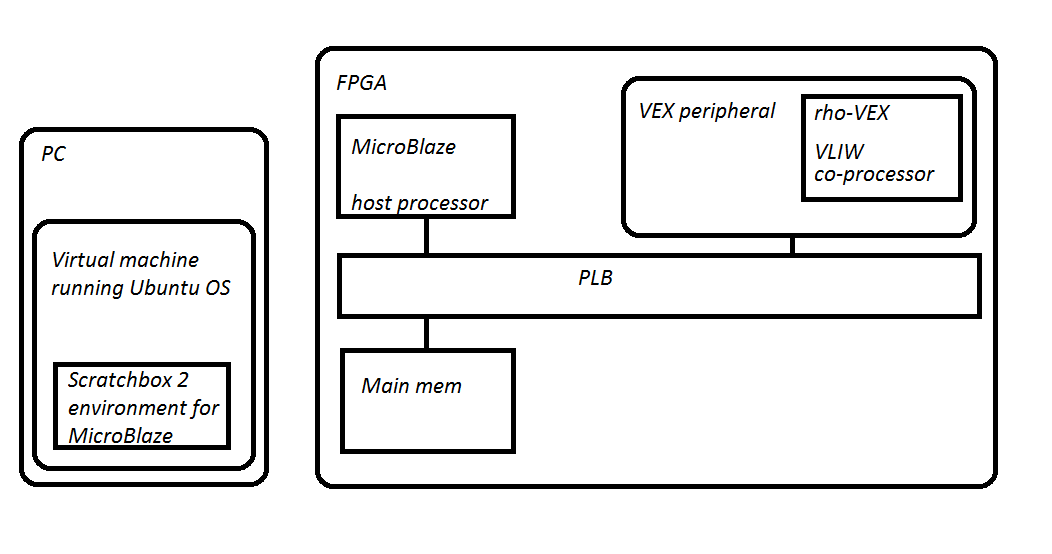
\includegraphics[width=\columnwidth]{Pictures/Platform_paint}%
\caption{Block diagram of the Virtual Machine and the ERA platform}%
\label{fig:lelijk}%
\end{figure}

In order to run the application on the MicroBlaze host processor, the \mcode{x264} executable must be compressed along with an input stream in a \mcode{tar.gz} file. This file can be put, via the FPGA host machine, on one of the three FPGAs using the \mcode{scp}, \mcode{ftp} and \mcode{put} command. For the programmer to connect to the development board, one must use the \mcode{ssh} and \mcode{telnet} command. See also fig \ref{fig:hoppen}.

% -- Plaatje Ubuntu-commando's ------------------------------
\begin{figure}[htb]%
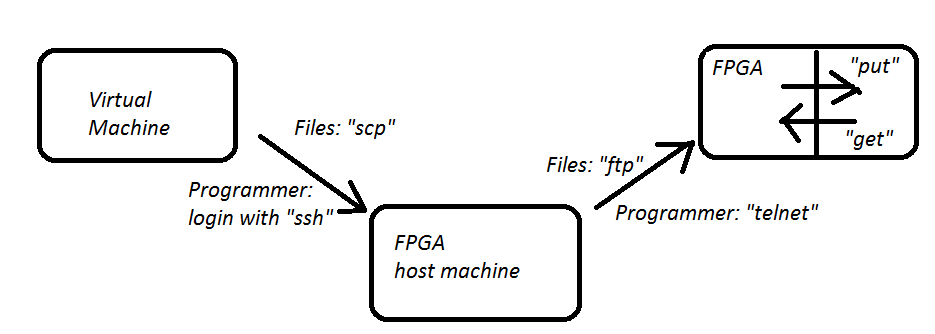
\includegraphics[width=\columnwidth]{Pictures/hop}%
\caption{Ubuntu commands for putting files on and navigating to the FPGAs}%
\label{fig:hoppen}%
\end{figure}

For the first lab, the \mcode{satd\_8x4} kernel has to be:
\begin{itemize}
	\item extracted into a separate file
	\item supplemented to a proper .c file which can be compiled and run using the $\rho$-VEX
	\item included in the makefile that creates a bytecode and bytedata file of the kernel
	\item debugged
\end{itemize}

Looking back, the debugging part has been chasing us all the way through the lab. Not only did we suffer from bugs in our source code, the $\rho$-VEX itself did also have shortcomings that had to be circumvented by downloading several fixes, competing for FPGA availability and break downs of the entire host machine due to unsufficient capacity for the amount of students.

